\documentclass{article}
% Language setting
% Replace `english' with e.g. `spanish' to change the document language
\usepackage[english]{babel}
\usepackage{url}
% \usepackage[numbers]

% \usepackage{subcaption}

\usepackage{float}

\usepackage[hidelinks]{natbib,hyperref}
\usepackage[top= 3cm, bottom=2cm, left=3cm, right=3cm]{geometry}
\usepackage{amsmath}
\usepackage{graphicx}
\usepackage{tikz}
\usepackage{nicefrac}




\graphicspath{{./images/}}

\pagestyle{myheadings}

\markright{Binary black hole detections\hfill 2663452m\hfill 12/04/2023\hfill}

\title{\textbf{Binary black hole detections from LIGO-VIRGO runs 1 and 2}}
\author{2663452m (University of Glasgow)}
\date{12/04/2023}



\begin{document}
\maketitle

\begin{abstract}
In this report the first ten Binary Black Hole merger events and the first neutron star merger event as
detected by the LIGO-VIRGO collaboration group are analysed and discussed obtaining estimates for the mass
pairs of each event, and distance, time and inclination of coalescence estimates and the associated errors. Starting with
event GW150914 with mass pairs of 36.06 $M_{\odot}$ and 35.76 $M_{\odot}$ and distance, time and inclination estimates of
1128 ± 82 Mpc, 3.198 ± 0.000 s and 0.03 ± 0.16 radians. Continuing the analysis for the rest of the events, handling the neutron star merger
seperately as it has different requirements and taking a closer look at the properties of the group of events.
\end{abstract}
\twocolumn
\newpage





\section*{Introduction and Background}
Gravitational waves as first predicted by Albert Einstein in 1915 in his paper on
special and general relativity, are ripples in the fabric of space-time due to the acceleration of large masses
and have been notoriously hard to detect. That was until
the LIGO Michelson interferometer in Hanford and Livingston was complete in 2015.
A Michelson interferometer is a device that uses the interference of two beams of
light to detect small changes in the path distance of the two. A diagram of one can
be seen in Figure 1.
\begin{figure}[h]
    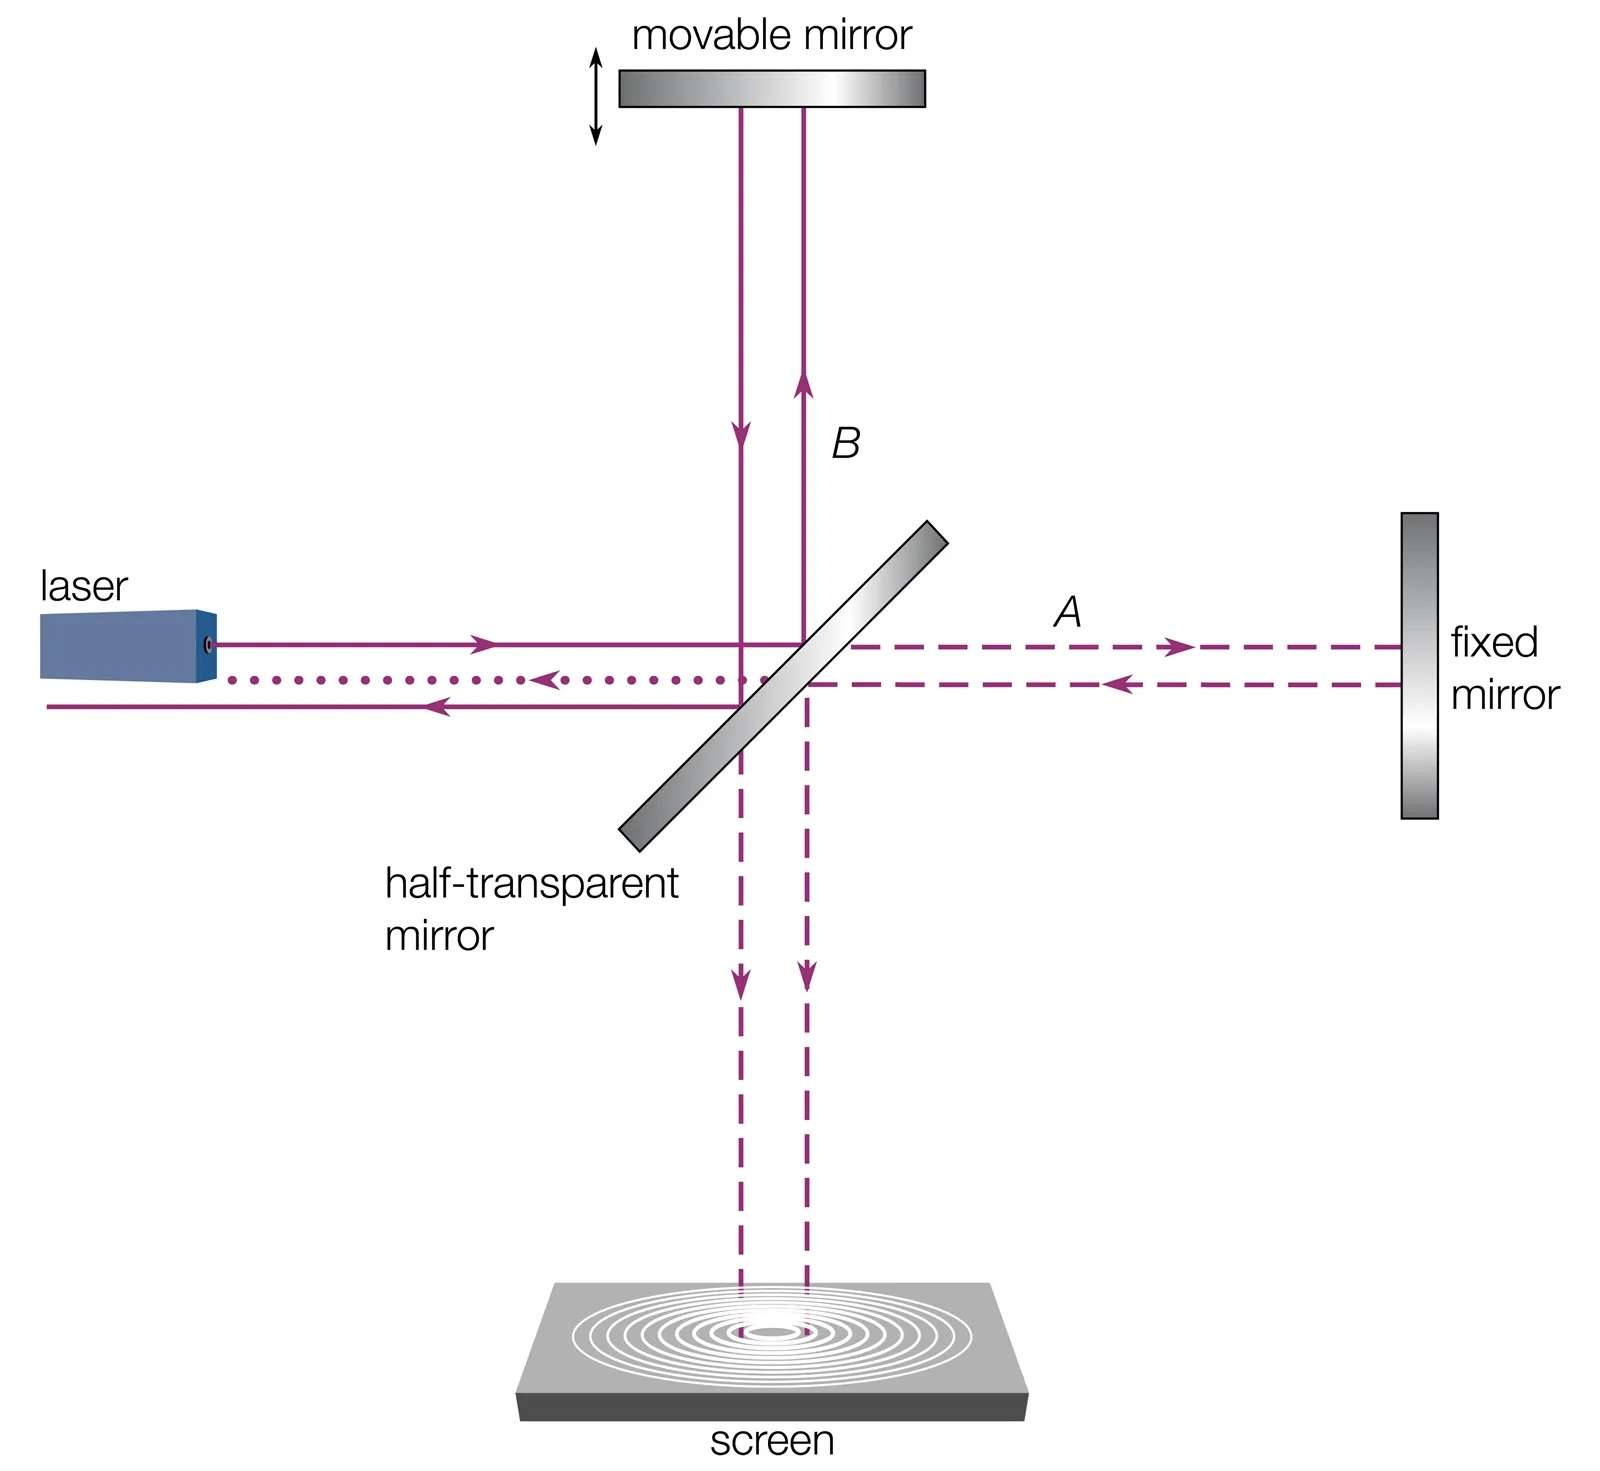
\includegraphics[width=6cm]{images/michelson_interferometer.png}
    \caption{Diagram of a michelson interferometer as used in LIGO.\cite{AZO}}\label{michelson}
\end{figure}
\newline
By using a Michelson interferometer in the LIGO experiment the small changes in
distance that are required can be detected and measured. These distances can be on the
order of 10$^{-21}$m this is called the strain of the wave and
is the amount of stretching over the original length and can be approximated as
\begin{equation}h
    \approx \frac{GM}{c^2d}\left(\frac{v}{c}\right)^2 \label{eq:strain}
\end{equation}
where $G$ is the gravitational constant, $M$ is the mass of the source, $c$ is the speed of light,
d is the distance to the source and $v$ is the velocity of the system.
\newline
This is caused by the passing of gravitational waves moving at the speed of light
through the
interferometer arms (which results in a shift in the interference pattern of the light beams).
The first detection of a gravitational wave was on the 14th of
September 2015, just 100 years after the publication of Einsteins paper.
The first detection was of a binary black hole merger, these mergers commonly
release a large amount of energy in the form of gravitational waves. This happens
because as the two black holes accelerate towards each other they warp the
space-time around them, and as they approach the point of coalescence the amplitude
of these waves massively increases, thus allowing them to be detected over the Background
noise. The ring-down after merging is extremely quick and thus leaving a distinct peak
at the time of coalescence. In this report the first 10 detections of gravitational waves
as a result of binary black hole mergers will be analysed and discussed alongside the first detection
of a binary neutron star merger that will be dealt with seperately starting with event GW150914.

\section*{Event GW150914}
To be able to carry out the analysis of the gravitaional waves it was necessary to set
up our workspace to be able to use some provided functions and packages written by the
LIGO collaboration. This was done by first installing the LIGO lalsuite package for Python 3.11
and then importing the packages into our notebook. The package contains a number of useful
functions that will be discussed in more detail later in this report.
For the first detection of gravitational waves GW150914 the data was provided
by the university through the Jupyter Hub. Once this data was loaded in
the first thing to do was identify by eye the peak
of the gravitational wave. The plot used to do this is shown in Figure 2.
\begin{figure}
    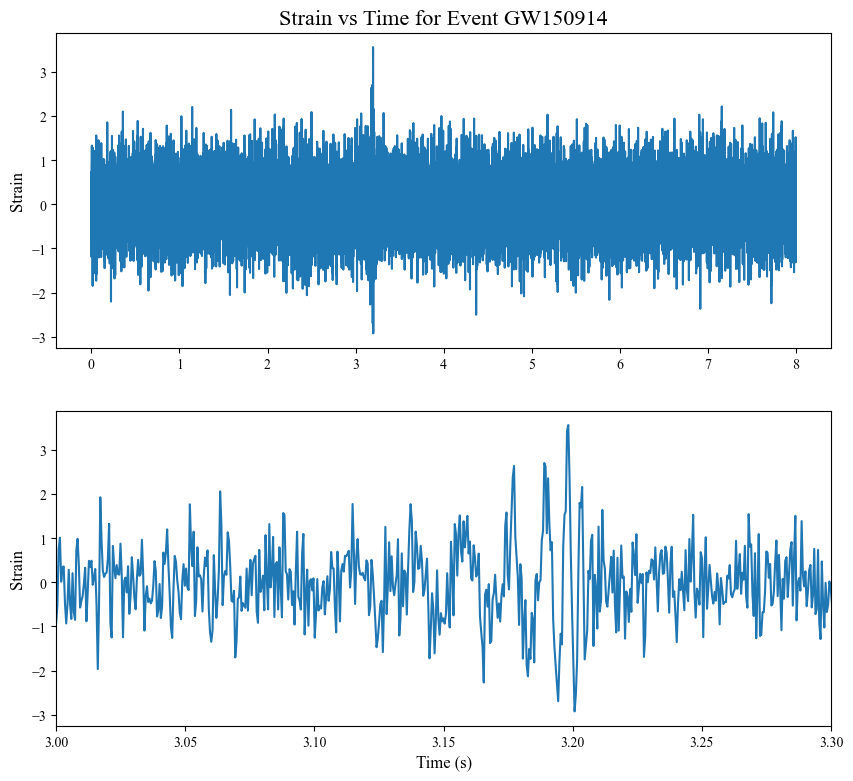
\includegraphics[width=6cm]{images/Signal_gw150914.png}
    \caption{top: Plot of the strain against time for GW150914 bottom:
    limited to shorter time to resolve the peak more.}
    \label{fig:GW150914}
\end{figure}

From Figure 2 it can be seen that the peak of the gravitaional wave occurs at
around 3.2 seconds.
Knowing this time we can use the SCIPY package to generate a spectrogram of strain and frequency and from this a color plot can be
created which visualizes the amount of energy in the gravitational wave at a given
frequency and time. This plot is shown in Figure 3.
\begin{figure}[h]
    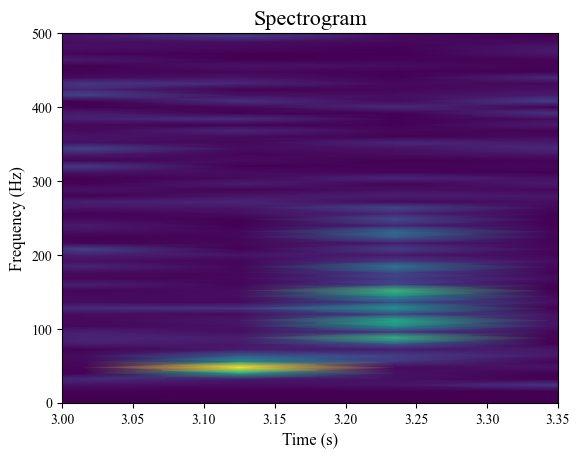
\includegraphics[width=6cm]{images/spectrogram_gw150914.png}
    \caption{Spectrogram of GW150914, showing the 'chirp' track of the gravitational wave.}
    \label{fig:spectrogram}
\end{figure}
\newline
In this plot the point where the energy is high across multiple frequencies
correlates with the same time as the peak in the strain in Figure 2, This confirms that the correct peak has been identified
in the given data and more analysis can be carried out on it.

Now that we have visualised the actual data from the gravitational wave, it would now
be useful to be able to compare this to the theorectical prediction of the event, this is necessary as it allows us
to use some estimating functions to determine values for the distance from earth that these events occured at as well as some
details about the coalescence, this is discussed below.
This can be generated using the make template function as supplied by the LIGO
collaboration. This function takes in the masses of the two black holes and
the time, frequency, distance and uncertainty on the data. The function then returns
a strain and time array that can be used to plot the theorectical predictions.
This produces an ideal signal as seen in Figure 4, this is easier to see the signal as
it no longer has any noise present in it.
\begin{figure}[h]
    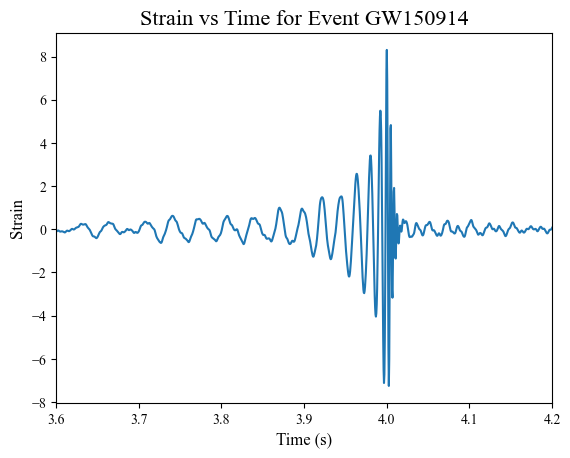
\includegraphics[width=6cm]{images/ideal_signal_gw150914.png}
    \caption{Theoretical prediction for GW150914}
    \label{fig:ideal_signal}
\end{figure}
\newline
Later this template will be overlayed on the true data to determine the goodness of fit.
\section*{Detecting the signals for the ten Black hole Mergers}
In this next section the detection of the signals will be looked at using some of the
techniques as discussed previously.

To determine the signal of the data for the ten black hole mergers the signal
to noise ratio (SNR) was used to determine the strength of the signal and its location in time.
This could be done using the function given in the lalsuite package. This function
returns a list of SNR's for each time in the data. If the SNR is low then the
template that was put into the function is badly aligned or the masses of the black holes
that were put into the template function are incorrect, and if the SNR is high
then the template is aligned well and the masses are correct. An example SNR time series
is shown in Figure 5.
\begin{figure}[h]
    \includegraphics[width=6cm]{images/SNR_gw150914.png}
    \caption{SNR time series for GW150914, with the peak at 3.2 seconds which tells
    us it is correctly aligned as this is the same time as obtained above}
    \label{fig:SNR}
\end{figure}
This SNR at the peak is important as it can be used later to determine the masses of the
black holes as well as other important information. So this value was stored to be used later.

\section*{Determining the masses of the black holes}
To determine the masses of the black hole pairs, some assumptions were made
about the system. The first assumption was that m1 the mass of the first black hole is larger
than m2 the mass of the second black hole. And the second assumption was that m1/m2 is less than 8
as this is the maximum mass ratio expected and it helps lower the number of possible mass pairs
for the next section. With these assumptions the mass of the black holes can be determined by
iterating over 10,000 possible mass pairs and calculating the SNR for each pair, then storing this
SNR and the corresponding mass pair. This was done for the 10 binary black hole mergers (the binary neutron star
merger was not included in this section as it has different mass ranges, and thus will be analysed seperately
later). With the SNR's and the mass pair options stored a color plot was created for each event, where
the intensity of the color is proportional to the SNR and the x and y axis are the mass of each black hole.
An example of one of these plots is shown in Figure 6.
\begin{figure}[h]
    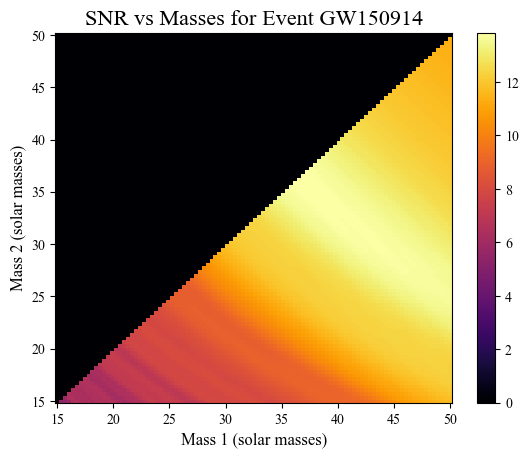
\includegraphics[width=6cm]{images/snr_color.png}
    \caption{Mass plot for GW150914, showing the mass pairs that give the highest SNR}
    \label{fig:mass_plot}
\end{figure}
\newline


\begin{table*}[h]
    \begin{center}
        \caption{Estimated values for the distance, time and inclination of coalescence and the mass pairs for the ten binary black hole mergers}
        \label{tab:estimates}
        \begin{tabular}{|c c c c c c|}
            \hline
            Event & Distance (Mpc) & Time (s) & Inclination (rad) & Mass one ($M_{\odot}$) & Mass two ($M_{\odot}$)\\
            \hline
            GW150914 & 1128 $\pm$ 82 & 3.198 $\pm$ 0.000 & 0.03 $\pm$ 0.16 & 36.06 & 35.76 \\
            GW151012 & 3783 $\pm$ 1677 & 2.703 $\pm$ 0.001 & 0.00 $\pm$ 0.82 & 35.40 & 11.72 \\
            GW151226 & 1812 $\pm$ 552 & 2.067 $\pm$ 0.000 & 0.00 $\pm$ 0.46 & 12.10 & 9.70 \\
            GW170104 & 2119 $\pm$ 340 & 1.975 $\pm$ 0.000 & 1.79 $\pm$ 0.32 & 35.86 & 25.35 \\
            GW170608 & 664 $\pm$ 81 & 3.794 $\pm$ 0.000 & 2.67 $\pm$ 0.18 & 11.27 & 8.36 \\
            GW170729 & 3150 $\pm$ 590 & 3.539 $\pm$ 0.001 & 2.89 $\pm$ 0.51 & 75.15 & 29.70 \\
            GW170809 & 2146 $\pm$ 444 & 2.641 $\pm$ 0.001 & 2.78 $\pm$ 0.42 & 46.41 & 15.10 \\
            GW170814 & 2268 $\pm$ 385 & 3.335 $\pm$ 0.000 & 0.00 $\pm$ 0.34 & 30.20 & 29.85 \\
            GW170818 & 1596 $\pm$ 417 & 2.161 $\pm$ 0.000 & 0.73 $\pm$ 0.40 & 12.79 & 9.91 \\
            GW170823 & 4111 $\pm$ 1121 & 4.456 $\pm$ 0.001 & 0.00 $\pm$ 0.64 & 55.25 & 26.26 \\
            \hline
        \end{tabular}

    \end{center}
\end{table*}

The black upper triangle is due to the conditional statement that mass one must be greater than mass two. Where the
color is the highest is where the SNR is highest and thus the mass pair that is most likely
to be correct. From this plot and as discussed above the mass pair that is most likely to
be correct is 36.06 and 35.74 solar masses. This is within estimated error of the masses published
by the LIGO collaboration of 35.6 and 30.6 solar masses. This method was repeated for the ten
black hole mergers considered in this report and the results are shown in Table 1.

\section*{Determining estimates for the distance, time and inclination of coalescence}



To find estimates for the distance, time and inclination of coalescence the make template function was used again
to generate a template for each event but this time using the masses as found above
as this would produce the most accurate templates for the sets of data.
From this the SCIPY curve fit function could be used as this allow for estimates of unknown quantities depending on the
how close the true data/plot is to the template. However for this particlar application
it was necessary to provide some upper and lower bounds that these value could take as this reduces the possible solutions
to the problem. These bounds were determined by looking at the peak and its location as well as an overall generic distance range
for the events. To help visualize this fitting of the data the plot of the generated template using these best estimates
overlayed on the raw data has bee included and can be seen in Figure 7.
How well these templates fit the raw data varied greatly for all the events as some couldn't identify the correct values
or the associated errors on these values were so large that it produced a graph that was severly off (these estimates were likely to be off
as the SNR for some events was too little to easily identify the true signal).

\begin{figure}
    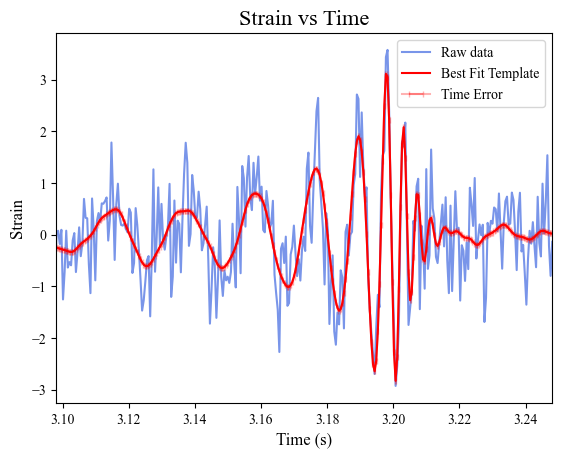
\includegraphics[width=6cm]{images/estimated_template.png}
    \caption{The template data as generated with the estimates for all values overlayed on the raw data}
    \label{fig:best_fit}

\end{figure}
The curve fit function also provides a covariance matrix which can be used to determine the error on the
estimated values. This was repeated for each event and the results are shown in Table 1 along with the mass estimates from the previous section.
It is worth noting here that the distance measurements as obtained in this analysis are incorrect when compared to the values published by the
LIGO-VIRGO collaboration group, however this appears to be a systematic error as for every event the
distance estimate is off by around 2-3 times the 'true' value. This is most likely the result of some systematic
error in the analysis that was completed, either a step was not included as it was beyond the skill level of this lab, or otherwise
this was due to not taking into consideration the inclination angle of the events, as this would also throw off the distance (for instance if a gravitational
wave propagates towards earth directly its strength will be at 100\%, whereas if the inclination angle as taken from the observing plane is at 45 degrees this
may be reduced to something like 50\% and if inclination angle is not considered this could appear to be a result of the distance therefore giving an estimate that is too large.)




\section*{The Binary Neutron star \newline merger GW170817}
As mentioned above the binary neutron star \newline merger was not included in the previous analysis as it has a different mass range that is required to be
searched over as well as some tighter parameters on the distance time and inclination of coalescence as it has an overall weaker signal and therefore
a worse SNR than the binary black hole mergers, making it more difficult to detect and requiring it to occur a lot closer to earth.
However, it is still possible to use the same methods as above to determine the masses of the neutron stars and the distance time and inclination of coalescence.
From this the following values were found as shown in Table 2.
\begin{table}[h]
    \begin{center}
        \caption{Estimated values for the distance, time and inclination of coalescence and the mass pairs for the binary neutron star merger GW170817}
        \label{tab:estimates}
        \begin{tabular}{|c c c c|}
            \hline
            GW170817 & Value & Error ±& Units\\
            \hline
            Distance & 92.0 & 17 & Mpc\\
            Time & 1.7 & 0.2 & s\\
            Inclination & 0.0 & 1.2 & rad\\
            Mass one & 1.63 & 0.00 & $M_{\odot}$\\
            Mass two & 1.16 & 0.00 & $M_{\odot}$\\
            \hline
        \end{tabular}

    \end{center}
\end{table}

From these values the mass ranges for neutron stars is obviously a lot lower then that for the
black hole mergers in the range of fractions of a solar mass up to about 5 solar masses,
and for this particular merger the masses were 1.63 and 1.16 solar masses, these values are very close to the
published values by the LIGO collaboration of 1.46 and 1.27 solar masses. For the results collected
in this analysis the errors on the distance time and inclination are higher than the general error as seen for the
black hole mergers, this as mentioned previously is because of the lower SNR and thus
it is more difficult to determine where the signal actually occurs in the data
and also to make accurate estimates using the same analysis techniques as
for the black hole mergers.
\section*{Properties of the events}
In this next section the 10 binary black hole events are going to be focused on and the binary
neutron star merger is once again going to be ignored as
it will only skew the results as for a neutron star merger to be detected it had to be extremely
close to earth due to the weakness f its signal and the masses in the pair are going to be
significantly lower then that of the black hole merger pairs.
\subsection*{The mass distribution of events}
\begin{figure}
    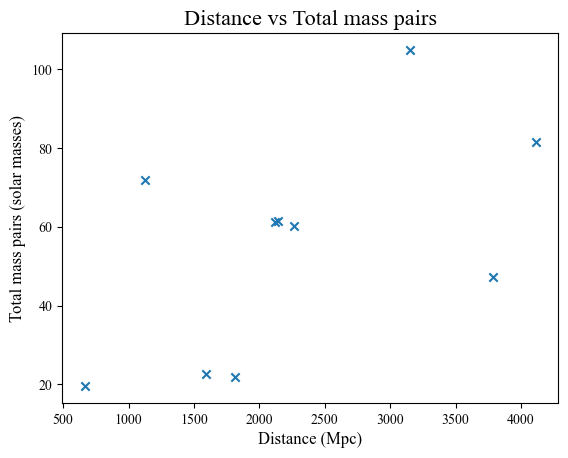
\includegraphics[width=6cm]{images/mass_pairs.png}
    \caption{Total mass of a merger as a function of its distance from earth}
    \label{fig:mass_pairs}
\end{figure}

When looking at the mass candidates for the binary black hole mergers, the individual masses are genrally in the region of
30-40 $M_{\odot}$ with some outliers as high as 76 $M_{\odot}$ and as low as 8.4 $M_{\odot}$, this upper limit is because as the masses increse the frequency of the emitted waves
decreases and on earth interferometers are not sensitive enough to be able to detect this. And the lower mass limit is due to the
formation of black holes as opposed to neutron stars, at around the 5-8 $M_{\odot}$ a star may collapse into either a neutron star or a black hole,
This limit alos arises due to the lower masses having weaker signals and therfore being harder to detect. The average total mass across
the ten events is 55.22 $M_{\odot}$ with a lowest mass pair of 19.63 $M_{\odot}$ and a highest
mass pair of 104.85 $M_{\odot} $ the total distribution can be seen in Figure 8.
The general trend of this plot is that for an increase in distance the mass pair is greater ($d \propto m $ where d is the distance to the source and m is the total mass of the system.)
This relation arises from the ability to detect these events, as for closer events it is more likely that lower mass candidates can be
detected due to the noise being lower over the shorter distance, where, as the distance increases these low mass pairs will be obscured by the background noise and only higher
mass pairs will be detectable.
\subsection*{Distance range of detected events}
Of the events discussed in this report the distance range that they occured in is relatively small only being a few thousand mega parsecs, detections closer to earth are unlikely however
as binary black hole systems form most commonly in regions of high stellar density which are generally far away, at least beyond the scope of the milky way galaxy.
the far distance limit however is most likely because of the decrease in the strength of the signal at such distances making these events more difficult to detect and the ground based interferometers
are not sensitive enough for this.

\section*{Conclusion}
The results obtained in this report for the masses, distance, time and inclinationof coalescence are all relatively accurate compared to the values
as published by the LIGO-VIRGO collaboration, this confirms that the analysis completed in this report is of substantial quality and takes enough precautions to
filter out edge cases. These results would be able to be used to go on and verify Einsteins ideas of general relativity, as well as confiming the effectiveness of these
detectors to go on and continue to detect new astrophysical objects to further our understanding of the universe and physics as a whole. This could potentially lead to
proving the existence of the graviton the ever elusive idea that the field force of gravity has some mediating particle.
To improve in these results more caution would be needed in the analysis of the neutron star source as it has high uncertainties and the optimisation function used is probably not
the most accurate so the develpoment of a function specifically for this use case may be useful. Another thing that would mprove the precision of the values obtained but not the
accuracy would be to have access to more computational power as this would allow for more iterations over the data and the use of more complex transforms.

\vspace{1cm}


\bibliographystyle{unsrt}%Used BibTeX style is unsrt
%\bibliography{sample}
%\begin{bibliography}
\bibliography{ref.bib}
\end{document}


